Events of interest in the HPS experiment are triggered by the ECal. Each channel of the ECal is readout to an FADC250 with 16 channels per board. The FADC250 continuously samples analog signals at a rate of 250~MHz, or every 4~ns with 12-bit precision. As the data size was small enough, the 2015 and 2016 data was recorded in raw mode such that 100~samples of raw information in a channel are read at the trigger time. This raw mode, called Mode 1, allowed for precise offline pulse fitting of the signals for optimal energy and timing resolution. In the 2015 Engineering Run, the signals from the ECal were split with $1/3$ of the signal going to TDCs and $2/3$ of the signal going to the FADCs. This was done as a precautionary measure in the event that the new FADCs were unreliable. In the 2016 Physics Run, the splitters were removed, allowing for the full signal to go to the FADC due to their proven capabilities. \\
\indent The full readout chain of the ECal trigger is shown in Figure~\ref{Figure:readoutChain}.
\begin{figure}[thb]
  \centering
      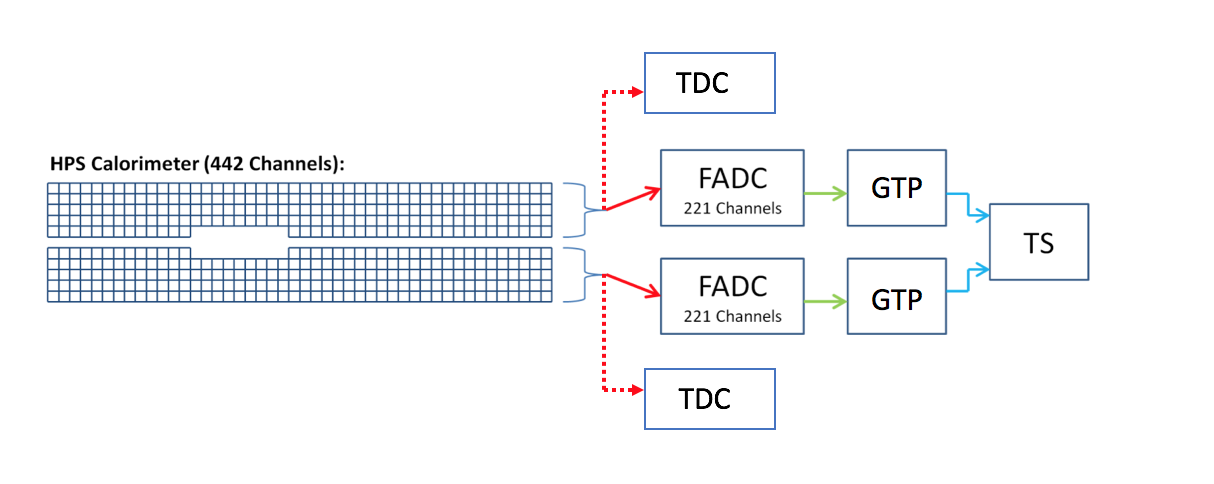
\includegraphics[width=0.75\textwidth]{pics/experiment/readoutChain.png}
  \caption[ECal readout chain]{The Flash ADC continuously samples ECal crystals at 250~MHz. In the 2015 Engineering Run, signals from the ECal were split with $1/3$ of the signal going to the TDCs and $2/3$ of the signal going to the FADCs. When a signal crosses threshold, the GTP makes $3\times3$ crystal clusters by searching for hits above threshold in adjacent crystals. The trigger processor (TP) uses the GTP clusters to make a trigger decision.}
  \label{Figure:readoutChain}
\end{figure}

When a signal crosses a pre-defined threshold, a set number of samples before and after the crossing are summed together to provide a pulse charge value which is converted to energy. The conversion to energy requires access to the individual channel gains and pedestals (as found by cosmic calibrations) which are pre-loaded into the data acquisition (DAQ) system. The energy and time of threshold crossing are sent to the General Trigger Processor (GTP) board every 16~ns  for clustering.~\cite{balossino_hps_2016}\\
\indent The GTP clusterer first identifies the crystal carrying the highest energy (known as the seed hit) in comparison to all surrounding crystals. The immediately neighboring crystals of the seed hit are compared in both energy and time coincidence with respect to the seed crystal in order to create a cluster. The cluster energy is the sum of all of the hits in a cluster. The timing coincidence is typically chosen to be 4~samples to allow for time-walk effects. The cluster information is then passed to the Subsystem Processor (SSP) to make a trigger decision based on various settable trigger cut requirements. \\
\indent The SSP includes several different trigger configurations that can run simultaneously containing different settable cuts and prescale values for ECal modules. The SSP looks for combinations of clusters that pass the configuration requirements and cuts and then sends a trigger to the Trigger Supervisor (TS) board when a cluster or pair of clusters satisfies the trigger requirements. The trigger is then sent to the Trigger Interface (TI) boards in order to trigger readout of all detectors.\\ 
\indent The SSP trigger configurations include two different cluster-pair triggers, two different single-cluster triggers, a random pulser trigger, a cosmic trigger, and an LED trigger of which all except for the cosmic and LED triggers were run during data taking with beam. The single cluster trigger, Single-1, was optimized for elastically-scattered beam energy electrons off the target. The looser version of the trigger was Single-0. These triggers were useful in selecting events for calibrating the ECal and studying the trigger efficiencies. The cluster-pair trigger is the primary trigger for the HPS experiment and studies all possible combinations of clusters in the ECal for pair selection. It requires one cluster in each half of the ECal. The tuneable cuts used in this trigger are presented in Table~\ref{tab:pairTriggerCuts}~\cite{balossino_hps_2016}. \\

\begin{table}[htb]
\caption{Pair-1 Trigger Cuts}
\label{tab:pairTriggerCuts}
\centering
\begin{tabular}{lc}
\toprule
%\multicolumn{2}{c}{Name} \\
%\cmidrule(r){1-2}
Trigger cut & Cut value \\
\midrule
Time difference & $| t_{top}-t_{bot} | \leq t_{coincidence}$   \\
Cluster energy & $E_{min}<E_{i}<E_{max}$\\
Cluster sum & $E_{sum min}\leq E_1+E_2\leq E_{sum max}$\\
Cluster size & $N_{hits}\geq N_{threshold}$\\
Energy difference & $ E_{2}-E_{1}<E_{difference}$\\
Coplanarity & $ |\arctan\dfrac{x_1}{y_1}-\arctan\dfrac{x_2}{y_2} | \leq \theta_{coplanarity}$\\
Energy-distance & $E_{1}+r_{1}F\geq E_{slope}$ \\ 
\bottomrule
\end{tabular}
\end{table}

The variables $t_i,E_i, N_i, x_i,$ and $y_i$ denote the cluster time, cluster energy, number of hits in the cluster, and coordinates of the cluster, respectively. The subscript, $1$, denotes the cluster with the lowest energy of the pair.  The parameter, $r_1$, is the distance between the center of the lowest energy cluster and the center of the ECal (defined as $r_1=\sqrt{x_1^2+y_1^2}$). The parameters selected for the cuts include the $t_{coincidence}, E_{min}, E_{max}, E_{sum min}, E_{sum max}, N_{threshold}, E_{difference}, \theta_{coplanarity}, r_{1},$ and $E_{slope}$, and are chosen from studying A$^{\prime}$ Monte Carlo in order to optimize the signal acceptance while minimizing the background. The GTP clusters are created prior to track-matching and offline clustering (which includes hits belonging to a cluster beyond those immediately adjacent to the seed hit). For the 2015 data, a GTP cluster conserves roughly 80$\%$ of the fully reconstructed particle energy when the seed hit is not on the edge of the ECal. \\
\indent The time coincidence cut is kept loose enough in the SSP pairs cluster selection to allow for time walk and cabling offsets which are not corrected for until the full pulse is fitted in offline reconstruction. At the GTP stage, the time only corresponds to threshold crossing. The cluster energy cut selects clusters that are reconstructed by the GTP in the energy range of interest. The minimum hit requirement for clusters was lowered at the start of running due to $A^{\prime}$ Monte Carlo studies indicating that 1 hit clusters were possible and could improve reach without overburdening the trigger. The cluster sum cut most significantly removes accidental pairs containing elastically-scattered beam energy electrons in addition to removing low energy cluster sum events that will not pass thresholds for well-reconstructed events. The energy difference cut removes events that have extremely different cluster energies and do not satisfy $A^{\prime}$-type criteria. \\
\indent The coplanarity cut removes events that are not coplanar including M$\o$ller and wide-angle bremsstrahlung (WAB) backgrounds because the $e^+e^-$ trident events of interest are distributed symmetrically around the beamline. The angle is calculated from the center of the ECal where the beam line passes through to each cluster in the pair relative to the vertical axis. The pairs should be approximately $180\degree$ apart. \\
\indent The energy-distance cut is applied to the lowest-energy cluster of the pair in order to reject events where the cluster is too close to where the electron beam passes through the ECal. Trident kinematics show that these clusters are dominated by bremsstrahlung low energy photons and that there is some reasonable distance of separation with respect to the beamline for these lower energy events. 
\indent The cut values used in the 2015 Pair-1 trigger are shown in Table~\ref{tab:pairTriggerVals}.

\begin{table}[htb]
\caption{Pair-1 trigger cut values for the Engineering Run}
\label{tab:pairTriggerVals}
\centering
\begin{tabular}{lc}
\toprule
%\multicolumn{2}{c}{Name} \\
%\cmidrule(r){1-2}
Trigger cut & Cut value \\
\midrule
Time difference & $| t_{top}-t_{bot} | \leq12$ ns   \\
Cluster energy & $54<E<630$ MeV \\
Cluster size & $N_{hits}\geq 1$\\
Energy sum & $180<E_{top}+E_{bot}<860$ MeV\\
Energy difference & $| E_{top}-E_{bot}|<540$ MeV\\
Coplanarity & $\theta_{top}-\theta_{bot}<30\degree $\\
Energy-distance & $E_{1}+(5.5 \textrm{ MeV/mm})r_{1}>600$ MeV\\ 
\bottomrule
\end{tabular}
\end{table}

\indent The pulser trigger generates a constant rate of triggers at 100~Hz regardless of the physics events as measured by the ECal. This makes the pulser an unbiased probe for measuring the backgrounds of the experiment during running with the beam and concurrent with other triggers.\\ 
\indent The cosmic trigger was used without the beam for calibration of the ECal and uses the timing coincidence between two scintillators, placed below and external to the ECal, in order to trigger readout of all ECal channels for offline reconstruction of the cosmic event. The timing coincidence of the scintillators placed in line and below the ECal was chosen to be 40~ns where the leading edge of the scintillator signal in the FADC pulse crosses 60~ADC samples. Once the timing and threshold conditions are met, all modules in the ECal were readout in Mode 1 format. 
